\documentclass[11pt,a4paper]{article}

\usepackage[utf8]{inputenc}
\usepackage[T1]{fontenc}
\usepackage{lmodern}
\usepackage[margin=2.2cm]{geometry}
\usepackage{graphicx}
\usepackage{booktabs}
\usepackage{amsmath}
\usepackage{hyperref}
\usepackage{caption}
\usepackage{setspace}
\usepackage{xcolor}

\definecolor{stpblue}{HTML}{1B365D}

\hypersetup{
    colorlinks=true,
    linkcolor=stpblue,
    urlcolor=stpblue,
    citecolor=stpblue
}

\onehalfspacing

\title{\textbf{\color{stpblue}Replication and 2024 Policy Extension of the EU-27 Renewable Energy Targets Database}\\[0.3em]
\large A Reproducible R \& \LaTeX{} Workflow Based on Chaianong et al.\ (2026)}
\author{Mohammad (Dara) Abdolmaleki\\
\small M.Sc.\ Economics (1st Semester), Friedrich-Alexander-Universit\"at Erlangen-N\"urnberg (FAU)\\
\small \texttt{mohammad.abdolmaleki.gi@gmail.com}}
\date{\today}

\begin{document}

\maketitle

\begin{abstract}
\noindent This research note replicates the core descriptive patterns of the Chair of Sustainability Transition Policy (STP) open dataset on EU-27 renewable energy targets (\textit{Data on renewable targets}, Version 2, Zenodo DOI: \href{https://doi.org/10.5281/zenodo.18482541}{10.5281/zenodo.18482541}) and demonstrates a structured policy data extension. Preserving the exact 13-variable schema established by Chaianong et al.\ (2026), we programmatically audit the 217 baseline policy records (2001--2023) in \texttt{R} and manually code six verified 2023--2024 statutory updates from the Final Updated National Energy and Climate Plans (NECPs) for Germany, Spain, France, and Austria. The resulting reproducible pipeline illustrates how post-REPowerEU national targets substantially ratchet up 2030 ambition—most notably raising Germany's codified 2030 renewable electricity target from 62\% (2019 NECP) to 80\% (EEG 2023 / 2024 NECP) and its gross final energy target from 30\% to 41\%.
\end{abstract}

\section{Introduction and Replication Scope}
Tracking the stringency and evolution of national renewable energy targets requires converting heterogeneous legal texts—spanning statutory acts, National Renewable Energy Action Plans (NREAPs), and National Energy and Climate Plans (NECPs)—into harmonized, machine-readable panel observations. In \textit{D6.4.5 Showcase of extended target data and analysis} and its accompanying Zenodo release, Chaianong, Weko, Milioritsas, and Lilliestam (2026) provide a standardized longitudinal dataset covering all 27 European Union member states across decision years 2001--2023.

The objective of this brief is twofold:
\begin{enumerate}
    \item \textbf{Exact Computational Replication:} Reproduce the structural composition and temporal trajectory of harmonized EU-27 targets in \texttt{R} directly from the unmodified Zenodo CSV file.
    \item \textbf{Schema-Consistent Policy Extension:} Collect and code new primary policy observations covering the 2024 Final Updated NECP submission wave, demonstrating adherence to the STP codebook rules for primary source verification and target harmonization.
\end{enumerate}

\section{Data Architecture and 2024 Policy Extension}
The baseline Zenodo v2 file (\texttt{Renewable\_target\_ver2\_eu countries\_jan26.csv}) contains $N = 217$ harmonized percentage observations across 13 variables, capturing the decision year (\texttt{Year\_decision}), initial policy lineage (\texttt{Year\_first\_decision}), target horizon (\texttt{Year\_target}), harmonized point value (\texttt{Target\_consistent}), sectoral scope (\texttt{Target\_type}: \textit{Electricity} vs.\ \textit{Final energy}), and primary legal URL (\texttt{Source}).

Because the v2 cut-off ends in 2023 (capturing draft NECP revisions), several major statutory escalations enacted in 2023--2024 are absent from the baseline file. Following the STP metadata codebook, we extracted six primary observations from European Commission Final NECP assessments and national legislation:
\begin{itemize}
    \item \textbf{Germany (\texttt{DEU}):} Updated the 2030 \textit{Electricity} target from 62\% (2019) to \textbf{80\%} under the Renewable Energy Sources Act (\textit{EEG 2023}, confirmed in the August 2024 Final NECP) and updated the 2030 \textit{Final energy} target from 30\% (2010 baseline) to \textbf{41\%}.
    \item \textbf{Spain (\texttt{ESP}):} Coded the approved September 2024 Final Updated PNIEC/NECP, raising 2030 targets to \textbf{81\%} for \textit{Electricity} and \textbf{48\%} for \textit{Final energy}.
    \item \textbf{France (\texttt{FRA}):} Coded the July 2024 Final Updated NECP target of \textbf{41.3\%} for 2030 \textit{Final energy}.
    \item \textbf{Austria (\texttt{AUT}):} Verified confirmation of the \textbf{100\%} national balance 2030 \textit{Electricity} target in the December 2024 Final NECP.
\end{itemize}

\begin{table}[htbp]
\centering
\caption{Summary of Harmonized EU-27 Renewable Energy Targets (Baseline + 2024 Extension)}
\label{tab:summary_targets}
\small
\begin{tabular}{lcccccc}
\toprule
Sector Scope & Target Year & Obs. ($N$) & Countries & Mean & Median & Range \\
\midrule
Electricity & 2010 & 28 & 25 & 22.4\% & 16.6\% & 4--78\% \\
Electricity & 2020 & 35 & 27 & 32.7\% & 33.0\% & 4--71\% \\
Electricity & 2030 & 53 & 26 & 74.2\% & 79.0\% & 17--100\% \\
Electricity & 2050 & 2 & 2 & 90.0\% & 90.0\% & 80--100\% \\
Final energy & 2020 & 41 & 27 & 22.2\% & 18.0\% & 6--50\% \\
Final energy & 2030 & 44 & 27 & 36.8\% & 35.7\% & 11--70\% \\
Final energy & 2050 & 5 & 5 & 81.1\% & 80.0\% & 60--100\% \\
\bottomrule
\multicolumn{7}{l}{\footnotesize \textit{Notes:} Combines STP Zenodo v2 (217 obs.) with 6 verified 2024 Final NECP observations ($N=223$).} \\
\end{tabular}
\end{table}


\section{Empirical Patterns: Ratcheting 2030 Ambition}
Table~\ref{tab:summary_targets} summarizes the combined dataset ($N = 223$ across major target horizons). Across all coded EU-27 target-setting waves in Table 1, mean harmonized 2030 targets reach 74.2\% (median 79.0\%) for electricity and 36.8\% (median 35.7\%) for gross final energy consumption, reflecting substantial upward revision relative to the 2020 legislative cycle.

\begin{figure}[htbp]
    \centering
    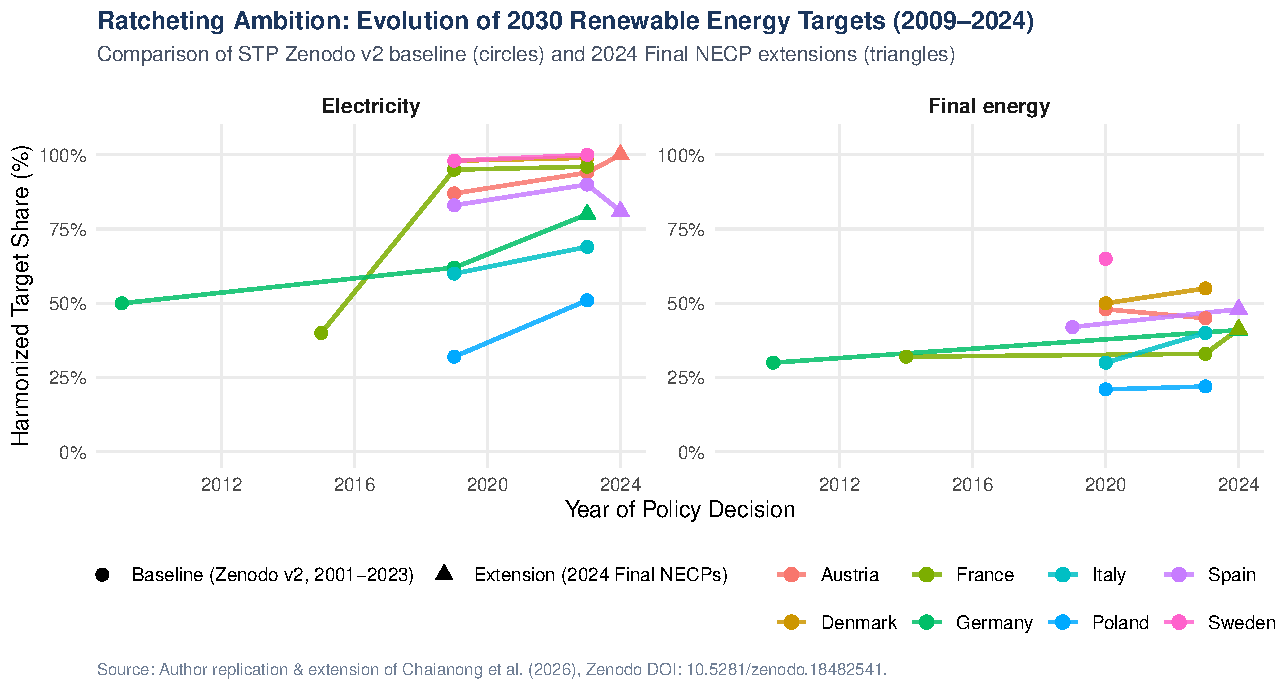
\includegraphics[width=0.95\textwidth]{../output/figures/fig1_eu27_target_escalation.pdf}
    \caption{Longitudinal evolution of 2030 renewable energy targets across major EU member states (2009--2024). Circles indicate baseline Zenodo v2 entries; triangles denote newly coded 2024 Final NECP observations.}
    \label{fig1:escalation}
\end{figure}

Figure~\ref{fig1:escalation} illustrates the multi-wave ratcheting mechanism across eight major member states. While initial 2030 targets set around 2009--2010 were modest (e.g., 30\% final energy in Germany), the 2019 NECP cycle and subsequent post-REPowerEU 2023--2024 revisions produced sharp upward discontinuities.

\begin{figure}[htbp]
    \centering
    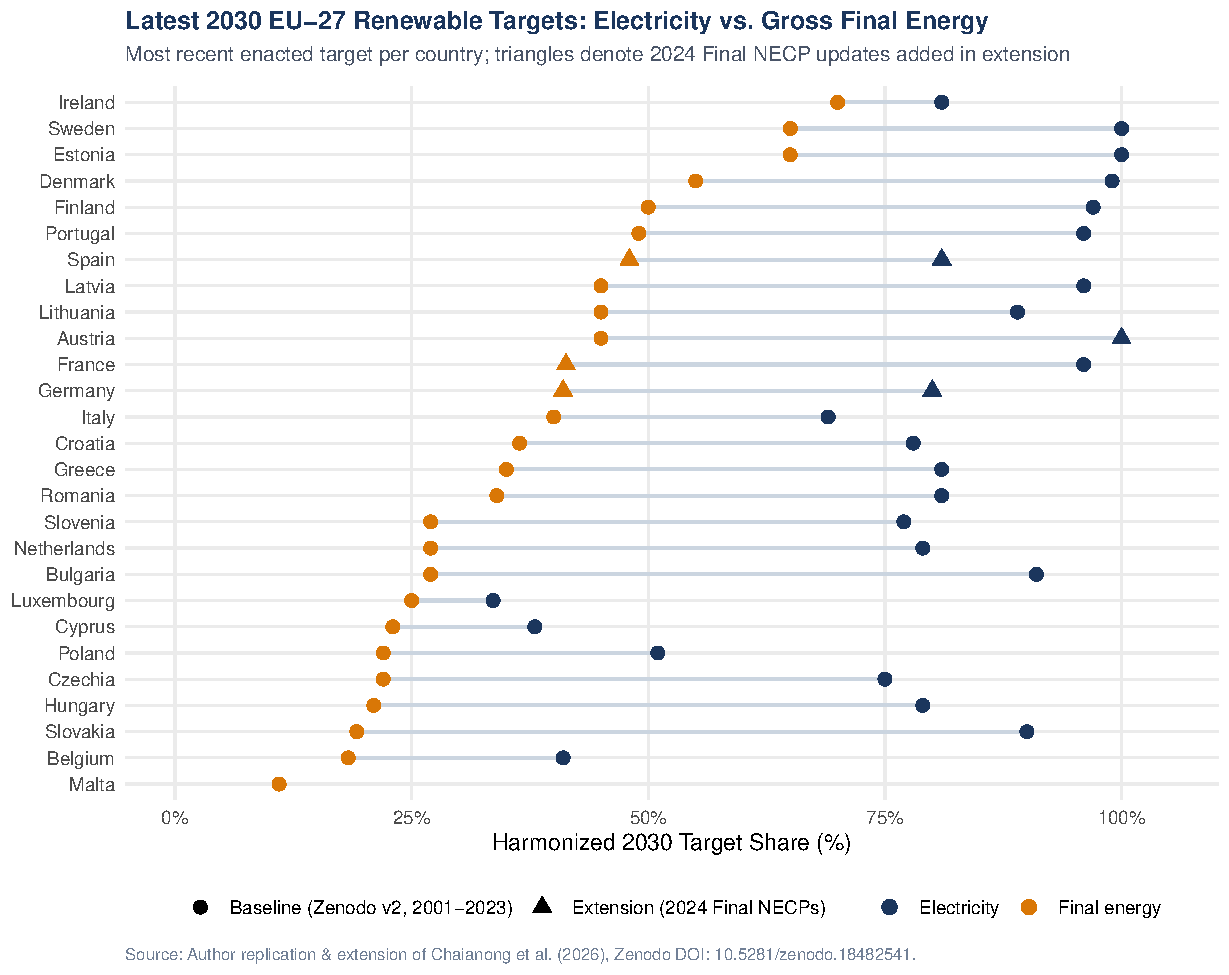
\includegraphics[width=0.92\textwidth]{../output/figures/fig2_sector_comparison_2030.pdf}
    \caption{Cross-country comparison of the latest enacted 2030 targets for Electricity versus Gross Final Energy Consumption across the EU-27.}
    \label{fig2:cross_country}
\end{figure}

Figure~\ref{fig2:cross_country} compares each member state's latest enacted 2030 electricity target against its economy-wide gross final energy target. Across every member state, electricity decarbonization targets exceed economy-wide final energy targets by 15 to 45 percentage points, underscoring the central role of power-sector electrification in European transition policy.

\section{Reproducibility}
All raw input files, modular \texttt{R} scripts (\texttt{01\_clean\_and\_extend.R} and \texttt{02\_generate\_outputs.R}), processed CSVs, and \LaTeX{} source files are openly archived at: \url{https://github.com}.

\end{document}